\RequirePackage{plautopatch}  % pLaTeX または upLaTeX のとき
%\documentclass[uplatex,dvipdfmx,titlepage,a4j]{jsarticle}% upLaTeX のとき
\documentclass[dvipdfmx,titlepage,a4j]{jsarticle}  % pLaTeX のとき
\usepackage{listings,jvlisting}
\usepackage{amsmath,amssymb}
\usepackage{graphicx}
\usepackage[yen]{okuverb}
\usepackage{r04ec-exp}
\usepackage{here}
\usepackage{ascmac}
\usepackage{fancybox}
\usepackage{fancyvrb}
\usepackage{fancyhdr}
\usepackage{lastpage}
\usepackage{cases}
\usepackage{url}
\usepackage[hang,small,bf]{caption}
\usepackage[subrefformat=parens]{subcaption}

\fancypagestyle{foot}
{
\fancyhead[C]{電気自動車充電器・メガソーラ発電設備等の高周波騒音の軽減}
\fancyhead[L]{}
\fancyhead[R]{}
\fancyfoot[C]{\thepage / \pageref{LastPage}}
\renewcommand\headrulewidth{0.4pt}
}

%ここからソースコードの表示に関する設定
\lstset{
  language={C++},
  basicstyle={\ttfamily},
  identifierstyle={\small},
  commentstyle={\smallitshape},
  keywordstyle={\small\bfseries},
  ndkeywordstyle={\small},
  stringstyle={\small\ttfamily},
  frame={tb},
  tabsize={2},
  breaklines=true,
  columns=[l]{fullflexible},
  numbers=left,
  xrightmargin=0zw,
  xleftmargin=3zw,
  numberstyle={\scriptsize},
  stepnumber=1,
  numbersep=1zw,
  lineskip=-0.5ex
}

\renewcommand{\lstlistingname}{リスト}
%ここまでソースコードの表示に関する設定

\title{フーリエ解析}
% 学年・番号
\grade{4年42番}%
% 氏名
\author{鷲尾 優作}
% 班(後期は班に分かれて実験をする.そのときは,ここに班番号を記入する.)
\team{}
% 提出日
\date{2023年1月31日}
% 実験日
\expdate{2023年1月5日,1月19日} 
% 共同実験者
% グループに分かれて実験をするテーマでは,グループメンバーの番号名前を書く.
\coauthor{
}
%
%記載例:
%\coauthor{%
%  2番 & 新潟 花子\\
%  11番 & 三条 次郎}
%%

\begin{document}
\pagestyle{foot}

\maketitle

\section{研究テーマ}
電気自動車充電器・メガソーラ発電設備等の高周波騒音の軽減

\section{背景・目的}
再生可能エネルギーの普及に伴い,日本各地で大電力を扱う設備が日常に溶け込む形で普及しつつあるなか,近年問題となっているのが励磁音である.
励磁音を発生させる代表的な装置であるパワコンユニットを備えた設備を図\ref{fig:reijion}に示す.

\begin{figure}[H]
  \centering
  \begin{minipage}{8cm}
    \centering
    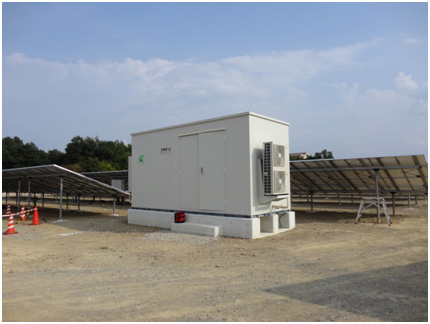
\includegraphics[keepaspectratio, scale=0.4]{../picture/z1.jpg}
    \subcaption{メガソーラー発電所のパワコンユニット}
  \end{minipage}
  \begin{minipage}{8cm}
    \centering
    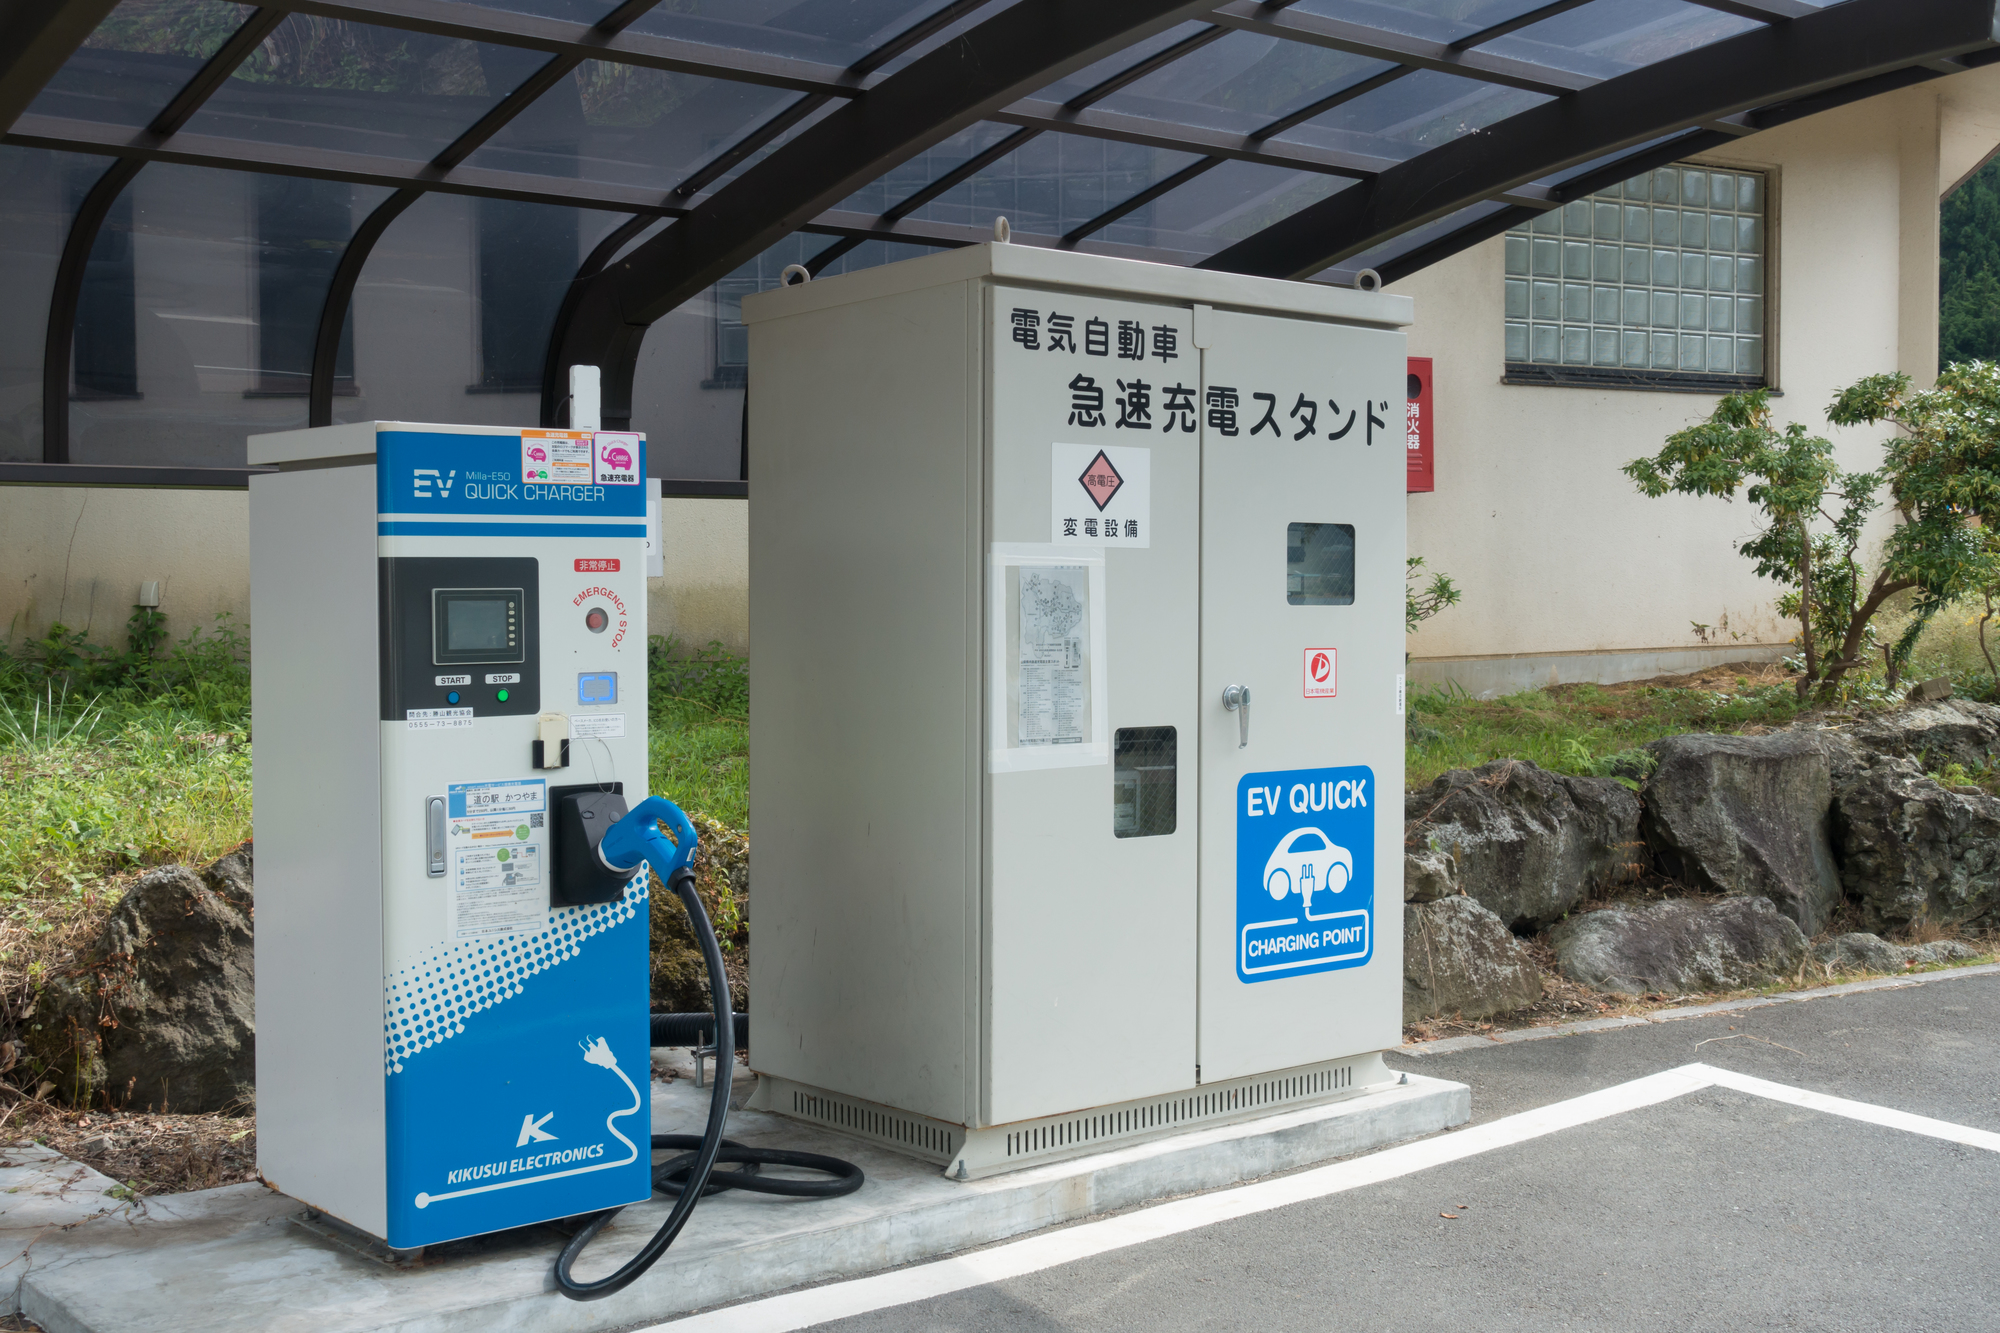
\includegraphics[keepaspectratio, scale=0.4]{../picture/pixta_38502286_M.jpg}
    \subcaption{電気自動車急速充電器}
  \end{minipage}
  \caption{励磁音の発生源}
  \label{fig:reijion}
\end{figure}

パワコンユニットは、送電ネットワークと蓄電に向いた直流の変換を担う装置である.
山間部のメガソーラー発電所のほか,都市部に設置された電気自動車急速充電器に使用され,動作中はキーンという高周波の音を発生させ,近隣住民とのトラブルの誘因に加え,生態系への影響も懸念されている.同様の家庭用設備では睡眠障害を引き起こすなど実生活に被害をもたらす問題であるといえる.

本実験では,生態系や人間の生活に対する発電設備の共存能力を向上させるため、励磁音の特性を解析し,騒音成分を軽減する方法を検討する.

\section{解析手法の検討}
\subsection{励磁音の発生源特定}

有効に励磁音を軽減するためには,励磁音の発生源を詳細に特定することが必要となる.
しかしながら本実験では,パワコンユニットを分解することは不可能であるため,パワコンユニットの内部にあるコイルや電極の振動を直接測定することは困難である.

一般的な考え方として,励磁音がパワコンユニットの内部にある複数のコイルや電極の振動によって発生していると仮定する.
この場合,パワコンユニット外部に流れる励磁音は,各発生源の振動によって発生する励磁音の和であると推定される.
今回はこの予測に基づき,パワコンユニット外部に流れる励磁音を測定し,フーリエ変換により励磁音の周波数特性を解析,発生源を特定することを目指す.

\subsection{離散フーリエ変換(DFT)}
コンピュータ上でフーリエ変換による周波数解析を実現する方法として,離散フーリエ変換(DFT)がある.
DFTは,本来連続関数に適用するフーリエ変換を,マイクロフォン等から取得した離散的な時系列データの解析に用いるためのアルゴリズムである.
実装が比較的容易であること,入力するデータの特性を考慮し,本実験ではDFTを用いて励磁音の周波数特性を解析する.

\paragraph{離散フーリエ変換の理論\\}
離散フーリエ変換の理論について述べる.
前提として連続関数に適用するフーリエ変換は,有限区間[$-T/2$, $T/2$]において式\ref{eq:fourier}で表される.
\begin{equation}
F(\omega) = \int_{-T/2}^{T/2} f(t) e^{-i\omega t} dt
\label{eq:fourier}
\end{equation}

しかしながら,離散的な時系列データに対して式\ref{eq:fourier}を適用すると積分計算が実施できず,0が出力されてしまう.
離散フーリエ変換は,この問題を解決するため入力信号のサンプリング周期に合わせ,複素フーリエ級数を用いて式\ref{eq:fourier}を近似するものである.
式\ref{eq:fourier}を複素フーリエ級数で近似すると,各周波数$\omega$におけるフーリエ成分$F(\omega)$は式\ref{eq:dft}で表される.
\begin{equation}
  F(\omega) = \sum_{n=0}^{N-1} f(n) e^{-i\omega n}
\label{eq:dft}
\end{equation}

\paragraph{アルゴリズムの実装\\}
上記アルゴリズムを実装するために,RustによるDFTの関数を作成した.Rustは,C/C++と同様に高速な実行速度を実現することができることに加え,メモリの安全性を保証することができる言語である.
将来的なFFTへの改造を考慮し,Rustを用いて実装した.
入力する時系列データは64bitの浮動小数点数を想定している.

リスト\ref{fourier.rs}に作成したRustによるDFTの関数実装を示す.

\lstinputlisting[caption=fourier.rs,label=fourier.rs,firstline=1,lastline=19,firstnumber=1,]
{../src/fourier.rs}

関数の入力と出力は,それぞれ入力信号$f(n)$と各周波数$\omega$におけるフーリエ成分$F(\omega)$とする.
関数の入力として,可変長の入力信号$f(n)$の時系列ベクタframesと入力信号のサンプリング周期sampling\_freqを与える.
関数の出力としては,可変長のComplexf64型のフーリエ成分を格納するベクタspectrumを返すものとする.


本関数は,リスト\ref{main.rs}に示すように実行する可能である.
実験中においては振幅スペクトルの大きさを補正するためにデータサイズの半分で割る処理が可能であるが,こちらは関数実装に含める必要性が薄いと判断し,
関数の返り値をここで補正する処理を実施している.

\lstinputlisting[caption=main.rs,label=main.rs,firstline=39,lastline=44,firstnumber=39,]
{../src/main.rs}

\section{環境}
本実験は次の環境で実施した.
\begin{itemize}
  \item PC: MacBook Pro Apple M1 16GB ( MacOS 13.1 )
  \item Rust: 1.52.1
  \item Python: 3.9.13 with anaconda
\end{itemize}

Rust依存環境
\begin{itemize}
  \item csv: 1.1.6
  \item ndarray: 0.15.6
  \item num: 0.4.0
\end{itemize}

\section{解析正当性の確認}
作成したRustによるDFTの関数が正しく動作しているかを確認するため,既知の正弦波の合成波形を入力し,応答を確認する.
ここでは,振幅5の波形を入力するものとし200Hzと1000Hzの正弦波の合成波を用いた評価をcase1,100Hz,500Hz,2000Hzの正弦波の合成波を用いた評価をcase2,case2のうち100Hzの振幅を2としたものをcase3とする.

解析データの評価を簡単とするため,同関数を呼び出しグラフ化するPythonのスクリプトを作成した.
スクリプトは,入力波形と計算後の振幅スペクトルをmatplotlibを用いて可視化するものである.
スクリプトを,リスト\ref{main.py},リスト\ref{main2.py}に示す.
本実験では,解析はこのスクリプトを通して実施する.

\lstinputlisting[caption=main.py,label=main.py,firstline=8,lastline=14,firstnumber=8,]
{../main.py}
\lstinputlisting[caption=main.py,label=main2.py,firstline=40,lastline=60,firstnumber=40,]
{../main.py}

\subsection{入力想定データ}
入力想定データとして,サンプリング周波数$8000$Hz,データ数$8000$個のデータを2つ用意しRustプログラムの正当性を評価した.
データは,1列目に時刻,2列目に振幅を格納したテキストファイルとして用意した.

case1で用いたデータの一部を参考として,リスト\ref{sin-200-1000.txt}に示す.
\lstinputlisting[caption=sin-200-1000.txt,label=sin-200-1000.txt,firstline=1,lastline=5,firstnumber=1,]
{../sin_200_1000.txt}

\subsection{case1 200Hzと1000Hzの正弦波の合成波}
case1で用いたデータを入力として,Pythonスクリプトを実行した応答を図\ref{case1}に示す.
処理は2.81秒で正常に終了した.
\begin{figure}[H]
  \centering
  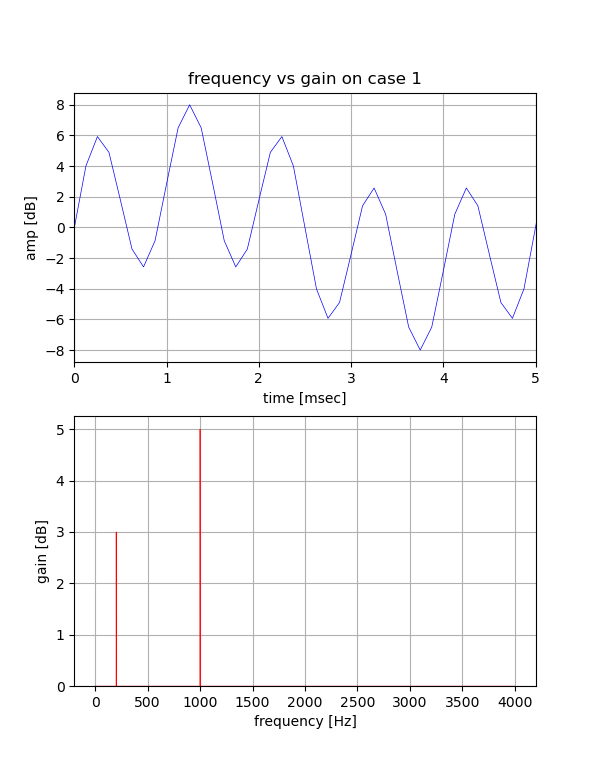
\includegraphics[width=0.4\linewidth]{../picture/case1.png}
  \caption{case1におけるDFT結果}
  \label{case1}
\end{figure}
図\ref{case1}からは,200Hzと1000Hzにピークを持つ振幅スペクトルが得られていることが確認できる.


\subsection{case2 100Hz,500Hz,2000Hzの正弦波の合成波}
case2で用いたデータを入力として,Pythonスクリプトを実行した応答を図\ref{case2}に示す.
処理は2.80秒で正常に終了した.
\begin{figure}[H]
  \centering
  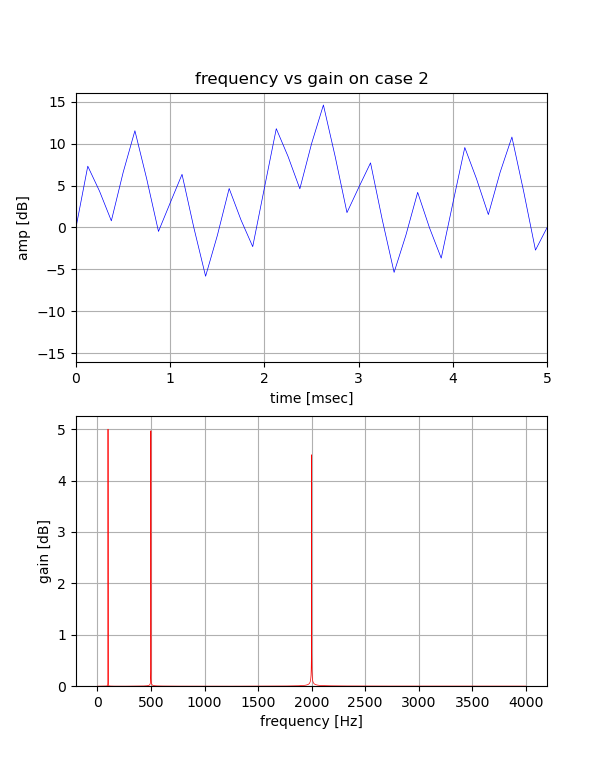
\includegraphics[width=0.4\linewidth]{../picture/case2.png}
  \caption{case2におけるDFT結果}
  \label{case2}
\end{figure}
図\ref{case2}からは,100Hz,500Hz,2000Hzにピークを持つ振幅スペクトルが得られていることが確認できる.
しかしながら,2000Hzの振幅が4.5とやや減少している.これはサンプリング周波数が8000Hzであるため,2000Hzの正弦波の周期が4サンプルとなりサンプリング定理は満たしているものの不足しているのではないかと考えられる.

\subsection{case2 100Hz,500Hz,2000Hzの正弦波の合成波 100Hzのみ振幅2}
case3で用いたデータを入力として,Pythonスクリプトを実行した応答を図\ref{case3}に示す.
処理は2.81秒で正常に終了した.
\begin{figure}[H]
  \centering
  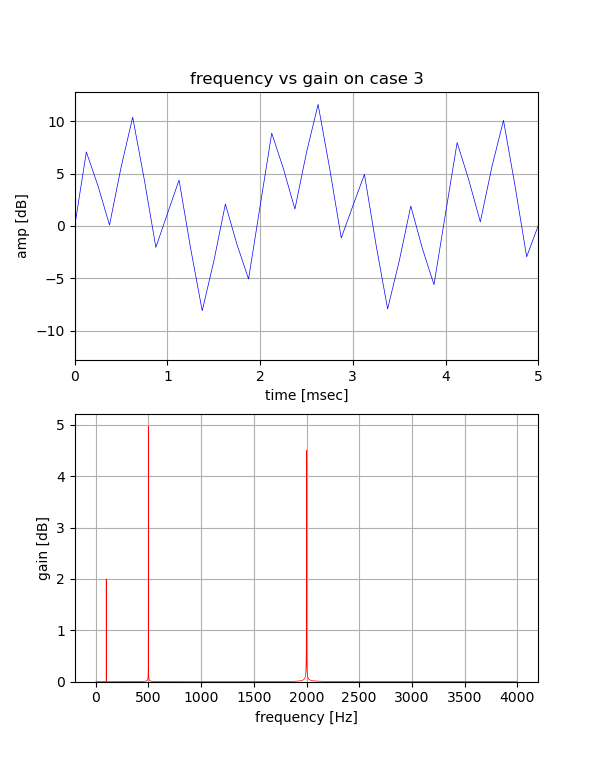
\includegraphics[width=0.4\linewidth]{../picture/case3.png}
  \caption{case3におけるDFT結果}
  \label{case3}
\end{figure}
図\ref{case3}からは,100Hz,500Hz,2000Hzにピークを持つ振幅スペクトルが得られており,100Hzの振幅が2になっていることが確認できる.

\subsection{結言}
case1,case2,case3ともに入力に対し意図した変換を実施でき,作成したRust関数および可視化用Pythonスクリプトを用いて,正弦波の合成波の振幅スペクトルを正しく計算することができたといえる.
case2,case3より,入力するデータの高周波領域の振幅については注意が必要であることがわかった.

\subsection{解析にかかる時間の確認}
作成したプログラムは,原理的には計算量オーダー$O(N^2)$である.ここでは,作成したプログラムの能力を確認するため,
Rustプログラムの解析開始から完了までの実行時間をPython側から測定し,グラフ化した.
図\ref{time}に示す.
\begin{figure}[H]
  \centering
  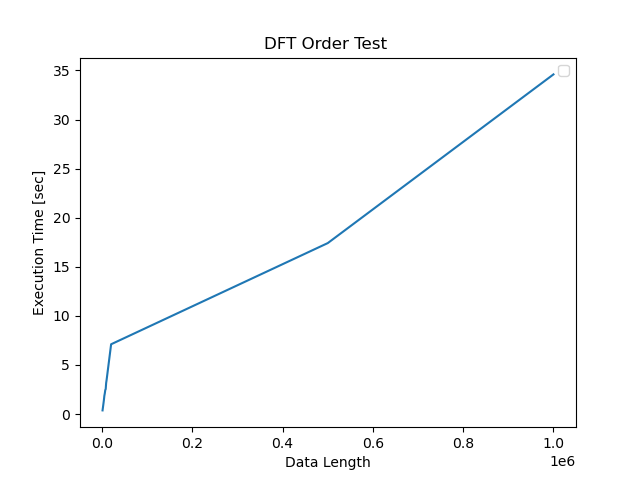
\includegraphics[width=0.5\linewidth]{../picture/order.png}
  \caption{解析にかかる時間}
  \label{time}
\end{figure}

図\ref{time}からは,解析にかかる時間は,入力データのサンプル数に対して,ほぼ$O(N)$とデータ数に対し効率が高すぎることがわかる.
原因については,不明であり,現在検討中である.

\section{実験方法}
具体的な実験の方法について述べる.

\subsection{データ取得}
実験に用いるデータは,既に取得済みのものを用いる.
データは新潟県の米山サービスエリアにて録音した電気自動車急速充電器の動作音である.
録音した音声データは,サンプリング周波数44100Hz,量子化ビット数16bitである.

取得時の条件を以下に示す.
\begin{itemize}
  \item 日時:2022年1月10日 19:00:48
  \item 録音機器:Apple iPhone XR
  \item 録音時間:約6秒
  \item 録音距離:約1m
  \item サンプリング周波数:44100Hz
  \item 録音位置:電気自動車急速充電器の側面
  \item 録音方法:動作中の急速充電器付近の地面にに録音機器を固定し取得.
\end{itemize}

\subsection{データの前処理}
\label{preprocess}
取得したデータは,そのままでは解析に用いることができないため,前処理を行う.
前処理は,以下の手順で行う.
\begin{enumerate}
  \item データをフリーソフトAudacity読み込む.
  \item データ中から周期関数としての特性を読み取り,1周期のみをトリミングする.
  \item データを1列目に時間,2列目に振幅を持つCSVファイルとして書き出す.
\end{enumerate}

\subsection{データの解析}
前処理を行ったデータを用いて,解析を行う.
解析は,以下の手順となる.
\begin{enumerate}
  \item CSVのURLをPythonスクリプトに渡す.
  \item PythonスクリプトがRustプログラムを呼び出し,データの周波数特性を解析する.
  \item Pythonスクリプトが,計算結果をグラフ化する.
  \item 数値を評価する.
\end{enumerate}

\section{測定結果}
測定対象の画像を図\ref{fig:sample}に示す.
\begin{figure}[H]
  \centering
  \includegraphics[width=0.5\linewidth]{../picture/obj.png}
  \caption{測定対象の画像}
  \label{fig:sample}
\end{figure}

電源周波数である50Hzを基準とし、N倍となる100Hz、200Hzなどの周波数が顕著に現れると予想し、測定対象の電気自動車急速充電器の動作音を測定した.
対象に対し、4度の測定を行い、中間の周期的と見られる波形に対し\ref{preprocess}章の手順を行った上で、フーリエ変換を行った.
順にSample1、Sample2、Sample3、Sample4とし、各サンプルのデータ数はそれぞれ400である.

図\ref{fig:sample1}、図\ref{fig:sample2}に解析結果を示す.

\begin{figure}[H]
  \begin{minipage}[b]{0.45\linewidth}
    \centering
    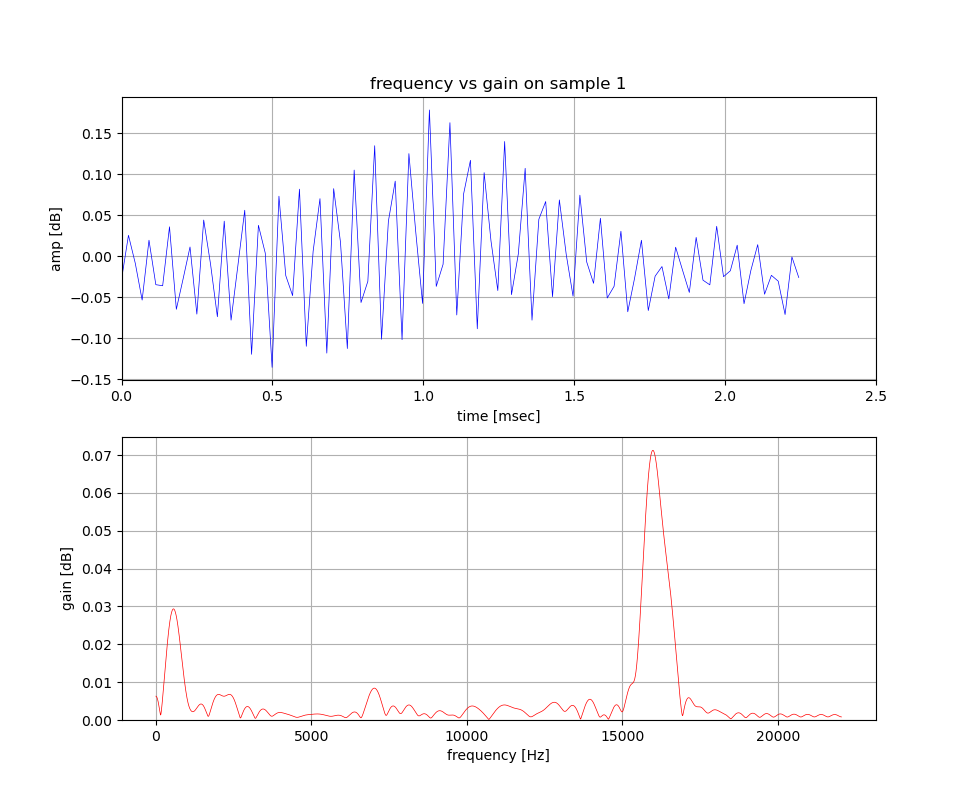
\includegraphics[scale=0.3]{../picture/1.png}
    \subcaption{Sample1}
  \end{minipage}
  \begin{minipage}[b]{0.45\linewidth}
    \centering
    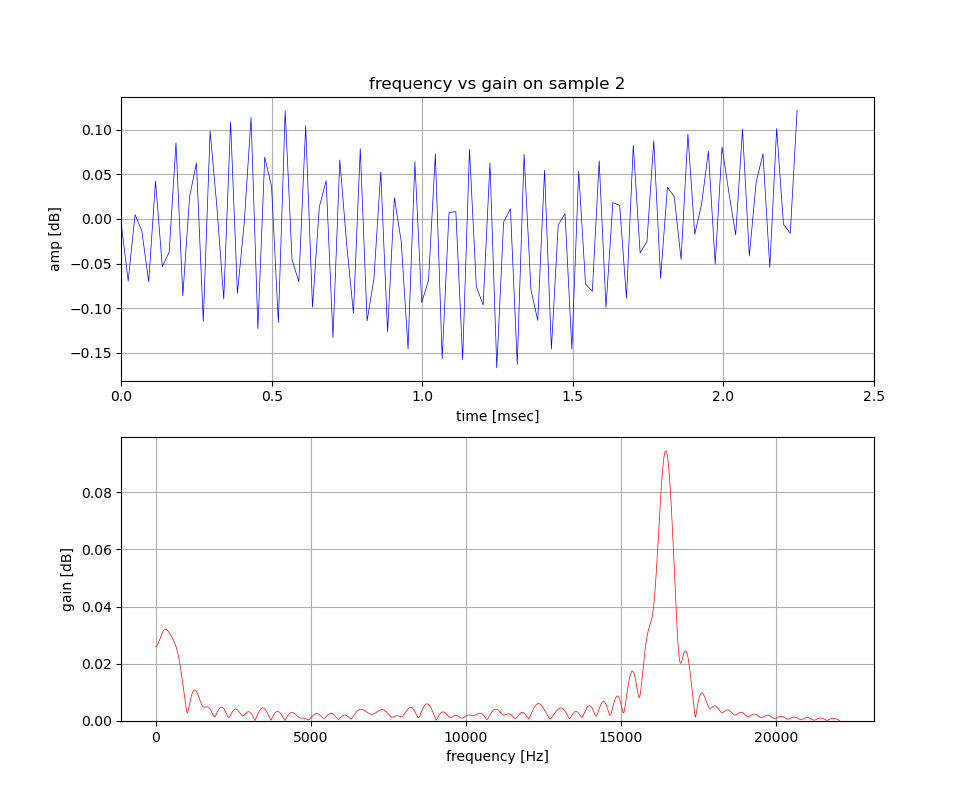
\includegraphics[scale=0.3]{../picture/2.png}
    \subcaption{Sample2}
  \end{minipage}
  \caption{Sample 1, 2の結果}
  \label{fig:sample1}
\end{figure}

\begin{figure}[H]
  \begin{minipage}[b]{0.45\linewidth}
    \centering
    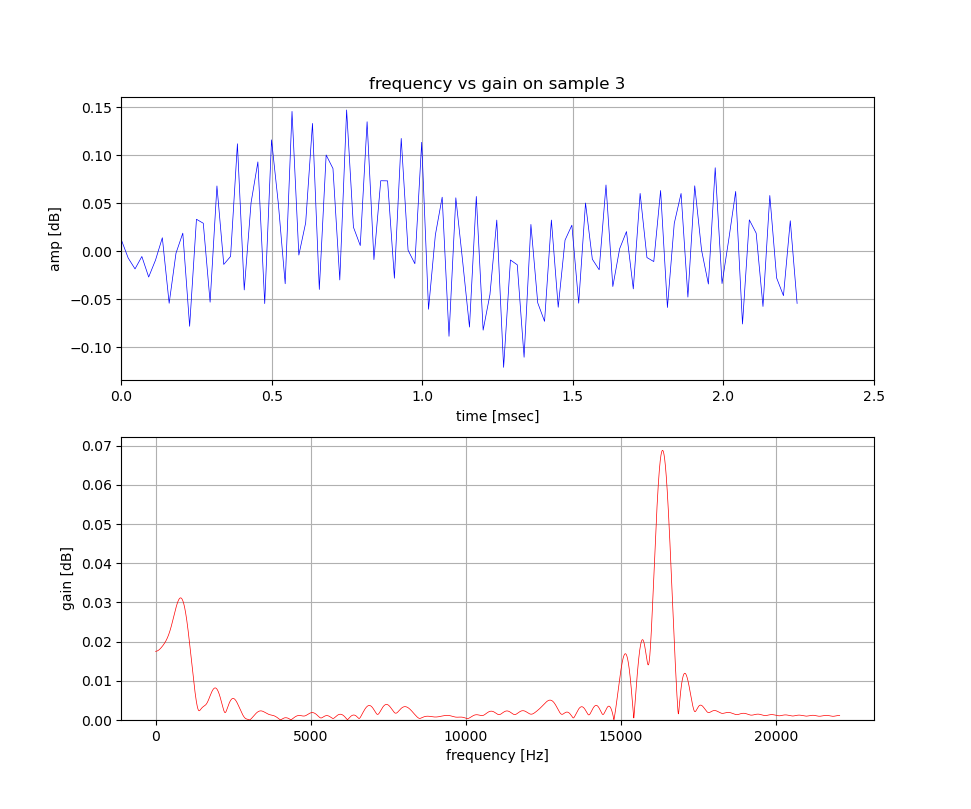
\includegraphics[scale=0.3]{../picture/3.png}
    \subcaption{Sample1}
  \end{minipage}
  \begin{minipage}[b]{0.45\linewidth}
    \centering
    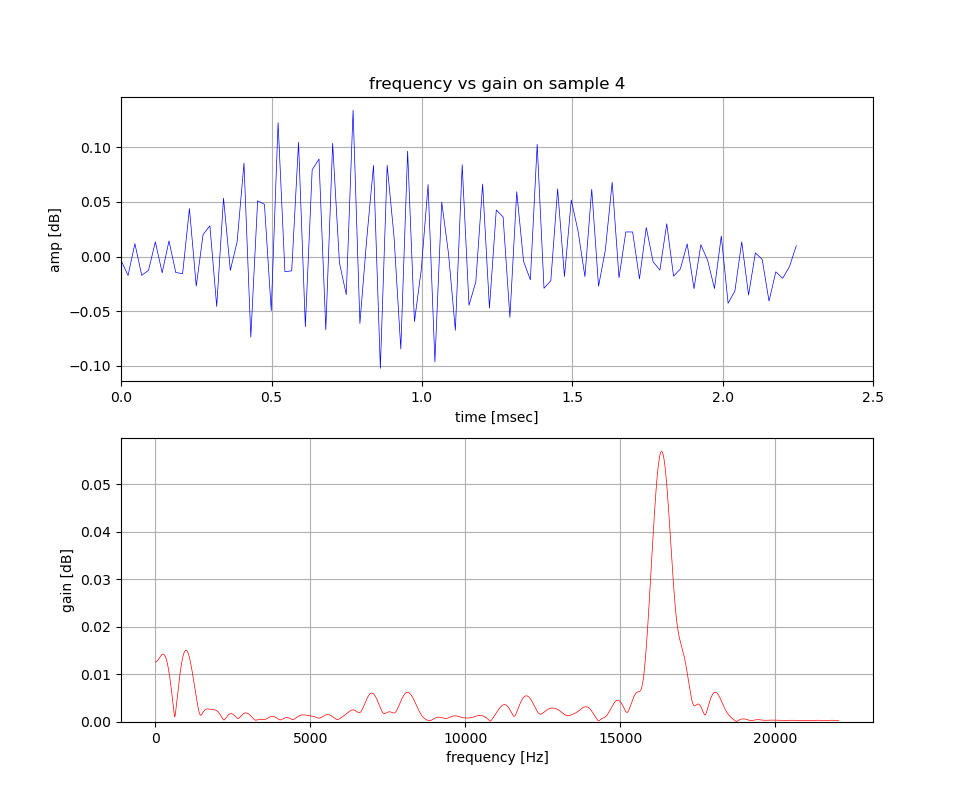
\includegraphics[scale=0.3]{../picture/4.png}
    \subcaption{Sample2}
  \end{minipage}
  \caption{Sample 3, 4の結果}
  \label{fig:sample2}
\end{figure}

各データより、高周波騒音の主な成分は15000Hzから20000Hzの間に分布していることがわかる.
Pythonスクリプトを作成し、各ピークの周波数を計算した.スクリプトをリスト\ref{maxvalue.py}、計算結果を\ref{table: peak}に示す.

\lstinputlisting[caption={maxvalue.py},label={maxvalue.py}]{../maxvalue.py}

\begin{table}[H]
  \centering
  \caption{ピーク周波数}
  \label{table: peak}
  \begin{tabular}{c|c|c|c|c|c}
    \hline\hline
    Sample & 1 & 2 & 3 & 4 & ave\\
    \hline
    Peak & 15985 & 16444 & 16339 & 16331 & 16274\\
    \hline
  \end{tabular}
\end{table}

表\ref{table: peak}より、ピーク周波数の平均値は16274Hzであり、この周波数に対する有効な騒音軽減方法を検討すれば良いことがわかる.

\section{騒音軽減方法の検討}
最も安価かつ効果的な騒音軽減方法として、騒音を吸収する材料を用いる方法を検討する.
騒音を吸収する材料として、木材やゴム、繊維素材などがある.
ここでは、吸音スポンジを例として、騒音軽減方法の検討を行う.

選定の結果、エンジンルーム用吸音素材「QonPET」が他の素材と比較して高周波領域の騒音吸収に有効であることがわかった.
図\ref{fig:qonpet}にQonPETの吸音特性を示す.\cite{online}

\begin{figure}[H]
  \centering
  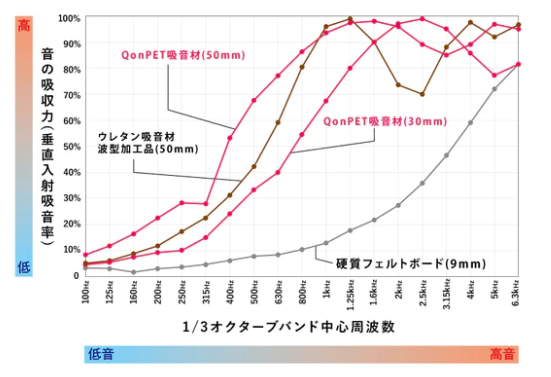
\includegraphics[width=0.5\linewidth]{../picture/qonpet.png}
  \caption{QonPETの吸音特性}
  \label{fig:qonpet}
\end{figure}

\section{結論}
本研究では、電気自動車急速充電器の高周波騒音を測定し、ピーク周波数を計算した.
計算結果より、ピーク周波数は16274Hzであることがわかった.
これに対し、吸音スポンジを用いた騒音軽減方法を検討し、QonPETが他の素材と比較して高周波領域の騒音吸収に有効であることがわかった.

しかしながら、より詳細な音響測定データをもつ吸音スポンジは主に4000Hzまでの周波数に対してデータシートを公開しており、
高周波領域の騒音吸収特性については不明であることから、「QonPET」以外の吸音スポンジを用いた騒音軽減方法の検討の価値は残されていると考える.

\section{終わりに}
今回、電気自動車急速充電器内部の回路についての検証は、内部回路図が得られなかったことより断念した.
周波数の高さから、電気自動車急速充電器の高周波騒音は、2次側によるものと考えられる.
今後もサンプルを増やし個人的に検証を続けていきたい.

\nocite{*}
\bibliographystyle{jplain}
\bibliography{refs}

\end{document}